\begin{name}
	{\tenchude}
	{TOÁN 11}
	{LỚP TOÁN THẦY PHÁT}
	{Thời gian: 90 phút - Không kể thời gian phát đề}
\end{name}
\TN
\Opensolutionfile{ans}[ans/ans-1-GK1-KNTT-14-NH23-24]
\begin{ex}%[0H3B6-2]% ::Cau 1::
	Với góc $\alpha $ bất kì, đẳng thức nào sau đây là đúng?
	\choice
	{$\cos \left( \pi-\alpha \right)=\cos \alpha $}
	{\True $\cos \left( \pi-\alpha \right)=-\cos \alpha $}
	{$\sin \left( \pi-\alpha \right)=-\sin \alpha $}
	{$\tan \left( \pi-\alpha \right)=\tan \alpha $}
	\loigiai{
		Ta có $\cos \left( \pi-\alpha \right)=-\cos \alpha $, $\sin \left( \pi-\alpha \right)=\sin \alpha $, $\tan \left( \pi-\alpha \right)=-\tan \alpha $.\\
		Do đó ta chọn phương án $\cos \left( \pi-\alpha \right)=-\cos \alpha $.}
\end{ex}
\begin{ex}%[0H3B5-2]% ::Cau 2::
	Biết góc $\alpha $ thỏa mãn $\cos \alpha =\dfrac{2}{3}$. Hỏi $\alpha $ có thể nhận giá trị trong khoảng nào dưới đây?
	\choice
	{$\left( \dfrac{\pi}{2};\dfrac{2\pi}{3} \right)$}
	{$\left( \dfrac{8\pi}{3};\dfrac{17\pi}{6} \right)$}
	{\True $\left( \dfrac{\pi}{4};\dfrac{\pi}{3} \right)$}
	{$\left( -\pi;-\dfrac{2\pi}{3} \right)$}
	\loigiai{
		Vì $\cos \alpha =\dfrac{2}{3}$ nên $\alpha \in \left( -\dfrac{\pi}{2}+k2\pi,\dfrac{\pi}{2}+k2\pi \right)$ với $k\in \mathbb{Z}$.\\
		Với $k=0$ thì $\alpha\in \left(-\dfrac{\pi}{2};\dfrac{\pi}{2}\right)$. Vì $\left( \dfrac{\pi}{4};\dfrac{\pi}{3} \right)\subset \left(-\dfrac{\pi}{2};\dfrac{\pi}{2}\right)$.\\
		Do đó, ta chọn phương án $\left( \dfrac{\pi}{4};\dfrac{\pi}{3} \right)$.}
\end{ex}
\begin{ex}%[0H3Y6-2]% ::Cau 6::
	Khẳng định nào sau đây là \textbf{sai}?
	\choice
	{$\cos a+\cos b=2\cos \dfrac{a+b}{2}\cos \dfrac{a-b}{2}$}
	{\True $\cos a-\cos b=2\sin \dfrac{a+b}{2}\sin \dfrac{a-b}{2}$}
	{$\sin a+\sin b=2\sin \dfrac{a+b}{2}\cos \dfrac{a-b}{2}$}
	{$\sin a-\sin b=2\cos \dfrac{a+b}{2}\sin \dfrac{a-b}{2}$}
	\loigiai{
		Theo công thức biến tổng thành tích ta có $\cos a-\cos b=-2\sin \dfrac{a+b}{2}\cdot\sin \dfrac{a-b}{2}$.}
\end{ex}

\begin{ex}%[1D1Y1-3]% ::Cau 9::
	Cho hàm số $y=\tan x$. Khẳng định sau đây là \textbf{sai}?
	\choice
	{\True Hàm số đã cho là hàm số chẵn}
	{Tập xác định của hàm số đã cho là $\mathbb{R}\setminus \left\{\dfrac{\pi}{2}+k\pi\,\middle|\, k\in \mathbb{Z} \right\}$}
	{Hàm số đã cho đồng biến trên mỗi khoảng $\left( -\dfrac{\pi}{2}+k\pi;\dfrac{\pi}{2}+k\pi \right)$ với $k\in \mathbb{Z}$}
	{Hàm số đã cho tuần hoàn theo chu kì $\pi$}
	\loigiai{
	Hàm số $y=\tan x$ là hàm số lẻ.
	}
\end{ex}
\begin{ex}%[1D1Y1-6]% ::Cau 10::
	Trong các hàm số sau, hàm số nào có đồ thị như hình vẽ bên dưới?
	\begin{center}
		\begin{tikzpicture}[scale=1,font=\footnotesize,line join=round,line cap=round,>=stealth]		
			\draw[-stealth] (-6.7,0)--(6.7,0)node[below]{$x$};
			\draw[-stealth] (0,-1.2)--(0,2)node[left]{$y$};
			\draw (0,0) node[below right]{$O$};
			\draw[thick,smooth,samples=200] plot[domain=-6.6:6.6] (\x,{sin (\x*180/pi)});
			\draw[fill=black]  (-6.28,0) circle (1pt) node [above left] {$-2\pi$};
			\draw[fill=black]  (-4.71,0) circle (1pt) node [below] {$-\dfrac{3\pi}{2}$};
			\draw[fill=black]  (-3.14,0) circle (1pt) node [above] {$-\pi$};
			\draw[fill=black] (-1.57,0) circle (1pt) node [above] {$-\dfrac{\pi}{2}$};
			\draw[fill=black]  (1.57,0) circle (1pt) node [below] {$\dfrac{\pi}{2}$};
			\draw[fill=black]  (3.14,0) circle (1pt) node [above] {$\pi$};
			\draw[fill=black]  (4.71,0) circle (1pt) node [above] {$\dfrac{3\pi}{2}$};
			\draw[fill=black]  (6.28,0) circle (1pt) node [above] {$2\pi$};
			\draw (0,1) node[above right] {$1$} (0,-1) node[below right] {$-1$};
			\draw[dashed] (-6.7,-1)--(6.7,-1) (-6.7,1)--(6.7,1);
			\draw[dashed] (-1.57,0)--(-1.57,-1) (1.57,0)--(1.57,1) (4.71,0)--(4.71,-1) (-4.71,0)--(-4.71,1);
		\end{tikzpicture}
	\end{center}
	\choice
	{\True $y=\sin x$}
	{$y=\cos x$}
	{$y=\tan x$}
	{$y=\cot x$}
	\loigiai{
		Từ hình vẽ ta thấy hàm số có miền giá trị từ $-1$ đến $1$, tuần hoàn với chu kỳ $2\pi$ và nhận gốc tọa độ làm tâm đối xứng nên đây là đồ thị của hàm số $y=\sin x$.}
\end{ex}

\begin{ex}%[1D1B2-1]% ::Cau 13::
	Giải phương trình $\cos \left( x-\dfrac{\pi}{6} \right)=\dfrac{1}{2}$.
	\choice
	{$\hoac{
			& x=\dfrac{\pi}{3}+k2\pi\\
			& x=k2\pi\\
		}\,\left( k\in \mathbb{Z} \right)$}
	{$\hoac{
			& x=\dfrac{\pi}{2}+k\pi\\
			& x=-\dfrac{\pi}{6}+k\pi\\
		}\left( k\in \mathbb{Z} \right)$}
	{$\hoac{
			& x=\dfrac{\pi}{2}+k2\pi\\
			& x=\dfrac{\pi}{6}+k2\pi\\
		}\left( k\in \mathbb{Z} \right)$}
	{\True $\hoac{
			& x=\dfrac{\pi}{2}+k2\pi\\
			& x=-\dfrac{\pi}{6}+k2\pi\\
		}\left( k\in \mathbb{Z} \right)$}
	\loigiai{
		Ta có $\cos \left( x-\dfrac{\pi}{6} \right)=\dfrac{1}{2}\Leftrightarrow \hoac{
			& x-\dfrac{\pi}{6}=\dfrac{\pi}{3}+k2\pi\\
			& x-\dfrac{\pi}{6}=-\dfrac{\pi}{3}+k2\pi\\
		}\Leftrightarrow \hoac{
			& x=\dfrac{\pi}{2}+k2\pi\\
			& x=-\dfrac{\pi}{6}+k2\pi\\
		}\left( k\in \mathbb{Z} \right)$.}
\end{ex}
\begin{ex}%[1D3B4-2]% ::Cau 17::
	Cho cấp số nhân $(u_n)$ với $u_1=-3;u_6=96$. Công bội của cấp số nhân đó là
	\choice
	{\True $q=-2$}
	{$q=-3$}
	{$q=2$}
	{$q=3$}
	\loigiai{
	Ta có $u_6=u_1q^5 \Rightarrow q^5=\dfrac{u_6}{u_1}=\dfrac{96}{-3}=-32$, suy ra $q=-2$.}
\end{ex}
\begin{ex}%::Cau 18::
	Công ty muốn ước lượng tỉ lệ các cỡ áo khi may cho học sinh lớp 11 đã đo chiều cao của 36 học sinh nam khối 11 của một trường và thu được mẫu số liệu sau (đơn vị là centimét):
	\begin{center}
		\begin{tabular}{lllllllllllll}
			160 & 161 & 161 & 162 & 162 & 162 & 163 & 163 & 163 & 164 & 164 & 164 & 164 \\ 
			165 & 165 & 165 & 165 & 165 & 166 & 166 & 166 & 166 & 167 & 167 & 168 & 168 \\ 
			168 & 168 & 169 & 169 & 170 & 171 & 171 & 172 & 172 & 174 & & & 
		\end{tabular}
	\end{center}
	Biết rằng học sinh có chiều cao thuộc $[160;167)$ sẽ mua cỡ áo M. Có bao nhiêu học sinh mua cỡ áo M?
	\choice
	{\True $22$}
	{$6$}
	{$15$}
	{$20$}
	\loigiai{
	Bảng tần số ghép nhóm
			\begin{center}
				\begin{tabular}{|c|c|c|c|c|c|}
					\hline Chiều cao $(\mathrm{cm})$ & {$[150 ; 160)$} & {$[160 ; 167)$} & {$[167 ; 170)$} & {$[170 ; 175)$} & {$[175 ; 180)$} \\
					\hline Số học sinh &0& 22 & 8 & 6 & 0 \\
					\hline
				\end{tabular}
			\end{center}
	}
\end{ex}
\begin{ex}%[0D5YC-2]% ::Cau 25::
	Thời gian xem ti vi trong tuần (đơn vị: giờ) của một số học sinh thu được kết quả như sau:
	\begin{center}
	\begin{tabular}{|c|c|c|c|c|c|}
		\hline
		Thời gian (giờ)	& $[0;4)$ & $[4;8)$ & $[8;12)$ & $[12;16)$ & $[16;20)$ \\
		\hline
		Số học sinh	& $6$ & $12$ & $4$ & $4$ & $2$ \\
		\hline
	\end{tabular}
	\end{center}
	Giá trị đại diện của nhóm $\left[ 12;16 \right)$ là
	\choice
	{$12$}
	{\True $14$}
	{$10$}
	{$16$}
	\loigiai{
	Giá trị đại diện của nhóm $\left[ 12;16 \right)$ là $\dfrac{12+16}{2}=14$.
	}
\end{ex}

\begin{ex}%[Dự án 1 - TLDH - TeamTeXHoa - Lê Quân]%[1K2B5-1] 
	Cho dãy số $(u_n)$ có $u_n=2\cdot 3^n$. Công thức truy hồi của dãy số $(u_n)$ là 
	\choice
	{$\heva{&u_1=6	\\&u_n=6u_{n-1},\, \forall n>1}$}
	{\True $\heva{&u_1=6	\\&u_n=3u_{n-1},\, \forall n>1}$}
	{$\heva{&u_1=3	\\&u_n=3u_{n-1},\, \forall n>1}$}
	{$\heva{&u_1=3	\\&u_n=6u_{n-1},\, \forall n>1}$}
	\loigiai{
		Ta có $u_n=2\cdot 3^n\Rightarrow \heva{&u_1=2\cdot 3^1=6	\\&u_{n+1}=2\cdot 3^{n+1}.}$\\
		$\Rightarrow u_{n+1}=2\cdot3\cdot 3^n =3u_n\Rightarrow u_n=3\cdot u_{n-1}$.\\
		Vậy $\heva{&u_1=6	\\&u_n=3u_{n-1},\, \forall n>1.}$
	}
\end{ex}
\begin{ex}%[Dự án 1 - TLDH - TeamTeXHoa - Sauluoi3105]%[1K2B5-4]
	Cho dãy số $\left(u_n\right)$, với $u_n=\dfrac{1}{1\cdot 4}+\dfrac{1}{2\cdot 5}+\ldots+\dfrac{1}{n(n+3)}, \forall n=1 ; 2 ; 3 \cdots$. Mệnh đề nào sau đây đúng?
	\choice
	{Dãy số $\left(u_n\right)$ bị chặn trên và không bị chặn dưới}
	{Dãy số $\left(u_n\right)$ bị chặn dưới và không bị chặn trên}
	{\True Dãy số $\left(u_n\right)$ bị chặn}
	{Dãy số $\left(u_n\right)$ không bị chặn}
	\loigiai{
		Ta có $u_n>0$ suy ra $\left(u_n\right)$ bị chặn dưới bởi $0$.\\ 
		Mặt khác $\dfrac{1}{k(k+3)}<\dfrac{1}{k(k+1)}=\dfrac{1}{k}-\dfrac{1}{k+1}\left(k \in \mathbb{N}^*\right)$ nên 
		$$u_n<\dfrac{1}{1\cdot 2}+\dfrac{1}{2\cdot 3}+\dfrac{1}{3\cdot 4}+\cdots+\dfrac{1}{n(n+1)}=1-\dfrac{1}{2}+\dfrac{1}{2}-\dfrac{1}{3}+\dfrac{1}{2}-\dfrac{1}{4}+\cdots+\dfrac{1}{n}-\dfrac{1}{n+1}=1-\dfrac{1}{n+1}<1.$$
Suy ra dãy $\left(u_n\right)$ bị chặn trên.\\
Vậy dãy $\left(u_n\right)$ bị chặn.
	}
\end{ex}
\Closesolutionfile{ans}
% \inputans{10}{ans/ans-1-GK1-KNTT-14-NH23-24}

\TNTF
\begin{ex}%[Thống kê – Trung bình và tứ phân vị]
Một công ty khảo sát mức chi tiêu (triệu đồng/tháng) của 150 khách hàng, kết quả được cho trong bảng:
\begin{center}
\begin{tabular}{|c|c|c|c|c|c|}
\hline
Khoảng chi tiêu & $[4;6)$ & $[6;8)$ & $[8;10)$ & $[10;12)$ & $[12;14)$ \\
\hline
Số khách hàng & $25$ & $40$ & $45$ & $30$ & $10$ \\
\hline
\end{tabular}
\end{center}
\choiceTF[t]
{\True Cỡ mẫu của mẫu số liệu là $150$}
{\True Giá trị trung bình của mẫu số liệu khoảng $8{,}8$}
{$Q_1 \approx 6{,}9$}
{$Q_3 \approx 10{,}7$}
\loigiai{
	\begin{itemchoice}
		\itemch Cỡ mẫu: $n = 25 + 40 + 45 + 30 + 10 = 150$.
		\itemch Giá trị đại diện các nhóm: $5; 7; 9; 11; 13$.\\
		Giá trị trung bình: $\overline{x} = \dfrac{5 \cdot 25 + 7 \cdot 40 + 9 \cdot 45 + 11 \cdot 30 + 13 \cdot 10}{150} \approx 8{,}8$.
		\itemch Tứ phân vị thứ nhất $Q_1$: $\dfrac{n}{4} = 37{,}5$. Nhóm $[6;8)$ chứa $Q_1$.\\
		$Q_1 = 6 + \dfrac{37{,}5 - 25}{40} \cdot 2 \approx 6{,}6$.
		\itemch Tứ phân vị thứ ba $Q_3$: $\dfrac{3n}{4} = 112{,}5$. Nhóm $[10;12)$ chứa $Q_3$.\\
		$Q_3 = 10 + \dfrac{112{,}5 - 110}{30} \cdot 2 \approx 10{,}17$.
	\end{itemchoice}
}
\end{ex}

\begin{ex}
	Cho hàm số $y=f(x)=\dfrac{\sin ^2x +1 }{\cos 2x}$. Khẳng định nào sau đây đúng?
	\choiceTF
	{Hàm số $y=f(x)$ có tập xác định là $ \left\{\dfrac{\pi}{4}+k\dfrac{\pi}{2},k\in \mathbb{Z} \right\}$}
	{\True Hàm số đã cho là hàm số chẵn}
	{$\sin^2x=\dfrac{1+\cos 2x}{2}$}
	{Đường thẳng $y=\dfrac52$ cắt đồ thị hàm số $y=f(x)$ tại vô số điểm có hoành độ dạng $x=\dfrac{\pi}{3}+k\pi,k\in \mathbb{Z}$}
	\loigiai{
		\begin{itemchoice}
			\itemch Hàm số đã cho xác định khi và chỉ khi $\cos 2x \ne 0 \Leftrightarrow 2x \ne \dfrac{\pi}{2} + k\pi \Leftrightarrow x \ne \dfrac{\pi}{4} + k\dfrac{\pi}{2}, k \in \mathbb{Z}$.\\
			Do vậy hàm số có tập xác định là $\mathbb{R}\setminus \left\{\dfrac{\pi}{4}+k\dfrac{\pi}{2},k\in \mathbb{Z} \right\}$.
			\itemch $\forall x \in \mathscr{D}, -x \in \mathscr{D}$, ta có
			$$f(-x) = \dfrac{\sin^2(-x) + 1}{\cos(-2x)} = \dfrac{\sin^2 x + 1}{\cos 2x} = f(x).$$
			Vậy hàm số đã cho là hàm số chẵn.
			\itemch Ta có $\sin^2 x = \dfrac{1 - \cos 2x}{2}$.
			\itemch Phương trình hoành độ giao điểm của đồ thị hàm số $y=f(x)$ và đường thẳng $y=\dfrac52$ là
			$$\dfrac{\sin^2 x + 1}{\cos 2x} = \dfrac52 \Leftrightarrow 1-\cos 2x - 5\cos 2x + 2 = 0 \Leftrightarrow \cos 2x = \dfrac{1}{2} \Leftrightarrow 2x = \pm \dfrac{\pi}{3} + k2\pi \Leftrightarrow x = \pm \dfrac{\pi}{6} + k\pi, k \in \mathbb{Z}.$$
		\end{itemchoice}
	}
\end{ex}

\TNSA
\begin{ex}
	Khai triển $\cos 4 \alpha$ theo $\cos \alpha$ ta được biểu thức $a\cos^4 \alpha +b\cos^2 \alpha +c$. Giá trị biểu thức $a-b+c$ bằng
	\shortans{17}
	\loigiai{
Ta có $\cos 4 \alpha =2\cos^2 2\alpha -1= 2 \left(2\cos^2 \alpha -1\right)^2 -1 = 8\cos^4 \alpha -8\cos^2 \alpha +1$.
}
\end{ex}
\begin{ex}%[1K1K4-3]%Câu 27
    Cho hai phương trình $\cos 3x-1=0$; $\cos 2x=-\dfrac{1}{2}$. Biết nghiệm chung của hai phương trình có dạng $x=\pm \dfrac{a\pi}{b}+kc\pi,k\in \mathbb{Z}$ với $a,b,c$ là các số nguyên dương và $\dfrac{a}{b}$ tối giản. Tính $a+b+c$.
	\shortans{6}
    \loigiai{
        Ta có 
        \begin{itemize}
            \item $\cos 3x-1=0\Leftrightarrow \cos 3x=1
            \Leftrightarrow x=k\dfrac{2\pi }{3}, k\in \mathbb{Z}$.
            \item $\cos 2x=-\dfrac{1}{2}
            \Leftrightarrow 2x=\pm \dfrac{2\pi }{3}+k2\pi \Leftrightarrow x=\pm \dfrac{\pi }{3}+k\pi,k\in \mathbb{Z}.$
        \end{itemize}
        Biểu diễn các nghiệm trên đường tròn lượng giác ta có tập các nghiệm của hai phương trình là $x=\pm \dfrac{2\pi }{3}+k\pi, k\in \mathbb{Z}$.}
\end{ex}

\begin{ex}%[1D3B3-5]% ::Cau 28::
	Cho cấp số cộng $\left( u_n \right)$ có $u_{27}+u_2=83$. Khi đó tổng $28$ số hạng đầu tiên của cấp số cộng $\left( u_n \right)$ là
	\shortans{1162}
	\loigiai{
		Gọi $d$ và $u_1$ lần lượt là công sai và số hạng đầu của cấp số cộng $\left( {u_n} \right)$\\
		Ta có $S_{28}=\dfrac{28\left( u_1+u_{28} \right)}{2}=\dfrac{28\left( u_2-d+u_{27}+d \right)}{2}=\dfrac{28\left( u_2+u_{27} \right)}{2}=\dfrac{28\cdot 83}{2}=1162$.}
\end{ex}

\begin{ex}%[1D3K3-4]% ::Cau 30::
	Cho $a<b<c$ là ba số nguyên. Biết $a$, $b$, $c$ theo thứ tự tạo thành một cấp số cộng và $a$, $c$, $b$ theo thứ tự tạo thành một cấp số nhân. Tìm giá trị nhỏ nhất của $c$.
	\shortans{2}
	\loigiai{
		Ta có $\heva{& 2b=a+c \\& c^2=ab>0}$. Suy ra $$2c^2=a\left( a+c \right)\Rightarrow 2c^2-ac-a^2=0\Rightarrow \hoac{
			& c=a\,\left( \text{loại} \right) \\
			& c=-\dfrac{a}{2}\Rightarrow b=\dfrac{a}{4}=-\dfrac{c}{2}.}$$
		Suy ra $a$, $b$ trái dấu với $c$ $\Rightarrow \heva{
			& a<0 \\
			& c>0.}$\\
		Do $a$, $b$, $c$ nguyên nên $c$ chia hết cho $2$.\\
		Do đó $c$ nhỏ nhất bằng $2$ khi đó $a=-4$, $b=-1$.}
\end{ex}

\TL
\begin{ex}%[1D1B2-1]% ::Cau 31::
	% \begin{enumEX}{1}
		% \item 
		Cho $\alpha \in (-\dfrac{\pi}{2};0)$ và $\sin \alpha = -\dfrac13$. Tìm $\cos \alpha$, $\tan \alpha$, $\cot \alpha$. 
		% \item Giải phương trình $\cot \left( 2x-40^{\circ} \right)=-\sqrt{3}$.
	% \end{enumEX}
	\loigiai{
		% \begin{enumEX}{1}
		% \item 
		Ta có $\alpha \in (-\dfrac{\pi}{2};0)$ nên $\cos \alpha >0$. Suy ra $$\cos^2 \alpha = 1-\sin^2 \alpha = 1-\left(-\dfrac13\right)=\dfrac89 \Rightarrow \cos \alpha = \dfrac{2\sqrt{2}}{3}.$$ 
		$\tan \alpha = \dfrac{\sin \alpha}{\cos \alpha} = \dfrac{-\dfrac13}{\dfrac{2\sqrt{2}}{3}}=-\dfrac{\sqrt{2}}{4}$.\\
		$\cot \alpha = \dfrac{1}{\tan \alpha} = -2\sqrt{2}$.
		% \item Ta có $\cot \left( 2x-40^{\circ} \right)=-\sqrt{3}\Leftrightarrow 2x-40^{\circ} =-30^{\circ} +k180^{\circ} \Leftrightarrow x=5^{\circ} +k90^{\circ} ,\,\left( k\in \mathbb{Z} \right)$.
	% \end{enumEX}
	}
\end{ex}

\begin{ex}%[1D3B3-3]% ::Cau 34::
	Tìm tổng $15$ số hạng đầu tiên của cấp số cộng $\left( {u_n} \right)$, biết $\heva{& u_1+u_5-u_3=10 \\& u_1+u_6=17.}$
	\loigiai{
	Ta có
		$$\heva{
			& {u_1}+u_5-u_3=10 \\
			& {u_1}+u_6=17}
		\Leftrightarrow \heva{
			& {u_1}+u_1+4d-\left( {u_1}+2d \right)=10 \\
			& {u_1}+u_1+5d=17}
		\Leftrightarrow \heva{
			& {u_1}+2d=10 \\
			& 2u_1+5d=17}
		\Leftrightarrow \heva{
			& u_1=16 \\
			& d=-3.}$$
		Suy ra $S_{15}=\dfrac{15}{2}\left(2u_1+14d\right)=\dfrac{15}{2}[2 \cdot 16 + 14\cdot (-3)]=-150$.}
\end{ex}

\begin{ex}%[1D1K3-8]% ::Cau 36::
	Hàng ngày mực nước của một con kênh lên xuống theo thủy triều. Độ sâu $h$ (mét) của mực nước trong kênh tính theo thời gian $t$ (giờ) $\left( 0\le t\le 24 \right)$ được mô tả bởi công thức $h=A\cos \left( \dfrac{\pi t}{6}+1 \right)+B$, với $A, B$ là các số thực dương cho trước. Biết độ sâu của mực nước lớn nhất là $15$ mét khi thủy triều lên cao và khi thủy triều xuống thấp thì độ sâu của mực nước thấp nhất là $9$ mét. Tính thời điểm độ sâu của mực nước là $13{,}5$ mét (tính chính xác đến $\dfrac{1}{100}$ giờ).
	\loigiai{
		Với mọi $0\le t\le 24$, ta có
		\allowdisplaybreaks
		\begin{eqnarray*}
		&& -1\le \cos \left( \dfrac{\pi t}{6}+1 \right)\le 1 \\
		&\Leftrightarrow& -A+B\le A\cos \left( \dfrac{\pi t}{6}+1 \right)+B\le A+B.
		\end{eqnarray*}
		Độ sâu của mực nước lớn nhất bằng $A+B$ khi $\cos \left( \dfrac{\pi t}{6}+1 \right)=1$ và thấp nhất bằng $-A+B$ khi $\cos \left( \dfrac{\pi t}{6}+1 \right)=-1$.\\
		Ta có hệ $\heva{
			& A+B=15 \\
			& -A+B=9}
		\Leftrightarrow \heva{
			& B=12 \\
			& A=3.}$\\
		Ta được $h=3\cos \left( \dfrac{\pi t}{6}+1 \right)+12$.\\
		Theo đề, ta tìm thời điểm mà độ sâu 
		\allowdisplaybreaks
		\begin{eqnarray*}
		&& h=13{,}5\Leftrightarrow 3\cos \left( \dfrac{\pi t}{6}+1 \right)+12=13{,}5\Leftrightarrow \cos \left( \dfrac{\pi t}{6}+1 \right)=\dfrac{1}{2}\\
		&\Leftrightarrow& \hoac{
			& \dfrac{\pi t}{6}+1=\dfrac{\pi}{3}+k2\pi\\
			& \dfrac{\pi t}{6}+1=-\dfrac{\pi}{3}+k2\pi},\left( k\in \mathbb{Z} \right)
		\Leftrightarrow \heva{
			& t=\left( -1+\dfrac{\pi}{3} \right)\cdot \dfrac{6}{\pi}+12k \\
			& t=\left( -1-\dfrac{\pi}{3} \right)\cdot \dfrac{6}{\pi}+12k},\left( k\in \mathbb{Z} \right).
		\end{eqnarray*}
		Do $0\le t\le 24; k\in \mathbb{Z}$ nên $t=0{,}09$ (giờ); $t=12{,}09$ (giờ); $t=8{,}09$ (giờ); $t=20{,}09$ (giờ).}
\end{ex}

	\begin{ex}%[Trần Ngọc Thành, CTST-BG11]%[1T3T1-6]
		Cho hình vuông $H_0$ cạnh bằng 1 đơn vị độ dài. Chia hình vuông $H_0$ thành chín hình vuông bằng nhau, bỏ đi bốn hình vuông, nhận được hình $H_1$. Tiếp theo, chia mỗi hình vuông của $H_1$ thành chín hình vuông, rồi bỏ đi bốn hình vuông, nhận được hình $H_2$. Tiếp tục quá trình này, ta nhận được một dãy hình $H_n$ $(n=1,2,3,\ldots)$.	
		\\
		\centerline{
			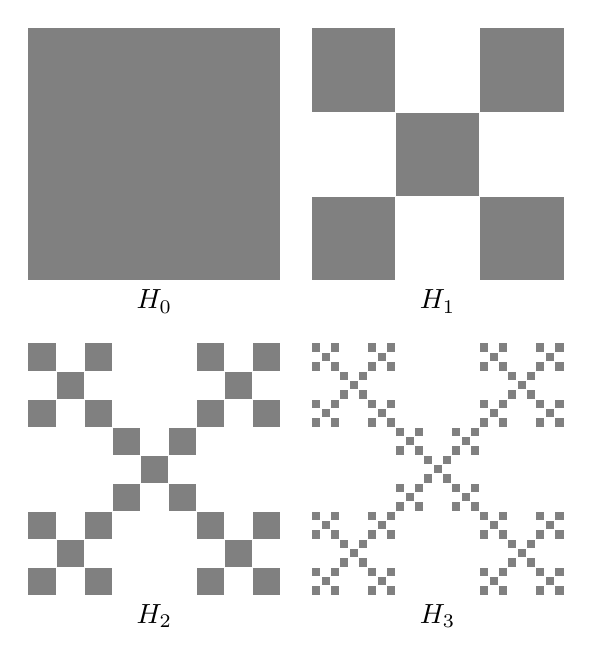
\begin{tikzpicture}[scale=.8]% Muốn vẽ hình Hn thì dùng \hv{n}
				\def\a{2}
				\pgfmathsetmacro\sh{2*\a *sqrt(2)/3}
				\def\hv#1{
					\ifnum#1>0
					\draw[white,fill=white] 
					(-\a/3,\a/3) rectangle (\a/3,\a)
					(-\a/3,-\a/3) rectangle (-\a,\a/3)
					(-\a/3,-\a/3) rectangle (\a/3,-\a)
					(\a/3,-\a/3) rectangle (\a,\a/3)
					;
					\pgfmathtruncatemacro{\k}{#1-1}
					\begin{scope}[scale=1/3]\hv{\k}\end{scope}
					\begin{scope}[shift={(45:\sh)},scale=1/3]\hv{\k}\end{scope}
					\begin{scope}[shift={(135:\sh)},scale=1/3]\hv{\k}\end{scope}
					\begin{scope}[shift={(225:\sh)},scale=1/3]\hv{\k}\end{scope}
					\begin{scope}[shift={(315:\sh)},scale=1/3]\hv{\k}\end{scope}
					\fi
				}
				\begin{scope}
					\fill[gray] (-\a,-\a) rectangle (\a,\a);
					\hv{0}
					\path (0,-\a)node[below]{$H_0$};
				\end{scope}
				\begin{scope}[xshift=4.5cm]
					\fill[gray] (-\a,-\a) rectangle (\a,\a);
					\hv{1}
					\path (0,-\a)node[below]{$H_1$};
				\end{scope}
				\begin{scope}[yshift=-5cm]
					\fill[gray] (-\a,-\a) rectangle (\a,\a);
					\hv{2}
					\path (0,-\a)node[below]{$H_2$};
				\end{scope}
				\begin{scope}[xshift=4.5cm,yshift=-5cm]
					\fill[gray] (-\a,-\a) rectangle (\a,\a);
					\hv{3}
					\path (0,-\a)node[below]{$H_3$};
				\end{scope}
				% \path (current bounding box.south) node[below]{Hình $6$};
			\end{tikzpicture}
		}
		Tính tổng diện tích và tổng chu vi tất cả hình vuông được tô màu trong hình $H_5$.
		\loigiai{
			\begin{enumerate}
				\item Hình vuông $H_1$ có diện tích $S_1=5\cdot \left(\dfrac{1}{3}\right)^2=\dfrac{5}{9}$.\\
				Hình vuông $H_2$ có diện tích $S_2=5^2\cdot \left(\dfrac{1}{3^2}\right)^2=\left(\dfrac{5}{9}\right)^2$.\\
				Hình vuông $H_n$ có diện tích $S_n=5^n\cdot \left(\dfrac{1}{3^n}\right)^2=\left(\dfrac{5}{9}\right)^n$.\\
				
				\item Hình vuông $H_1$ có chu vi $C_1=5\cdot 4\cdot  \dfrac{1}{3}=4\cdot \dfrac{5}{3}$.\\
				Hình vuông $H_2$ có chu vi $C_2=5^2\cdot4\cdot \dfrac{1}{3^2}=4\cdot \left(\dfrac{5}{3}\right)^2$.\\
				Hình vuông $H_n$ có diện tích $C_n=5^n\cdot4\cdot  \dfrac{1}{3^n}=4\cdot \left(\dfrac{5}{3}\right)^n$.\\
				
			\end{enumerate}
			Vậy $S_5=\left(\dfrac{5}{9}\right)^5$ và $C_5=4\cdot \left(\dfrac{5}{3}\right)^5$.
		}
	\end{ex}
